\section{Problema 1: Tel\'egrafo}

\subsection{Descripci\'on de la problem\'atica}

En el primer ejercicio se nos presenta un contexto en el que se pretende conectar con un cable de longitud arbitraria la mayor cantidad de estaciones férreas consecutivas pertenecientes a un ramal dado. 
Siéndonos provistas las distancias entre las sucesivas estaciones y la longitud del cable, la propuesta de este problema es hallar el valor de dicha cantidad.

Supongamos, por ejemplo, que nos fuera dado un ramal con cada estación  0<$i$ definida en el kilometro $j*2+2^(j-1)$ de manera tal que en un ramal de cinco estaciones las mismas se encontraran en los kilómetros 0, 3, 6, 10, 16.
Si contáramos con un cable de 5 kilómetros, la respuesta correcta debería ser "2", puesto que con dicha longitud se podrían unir a lo sumo dos estaciones (pudiendo ser las mismas la primera y la segunda, la segunda y la tercera o la tercera y la cuarta).
Si el mismo cable pudiera extenderse hasta los 6 km, la respuesta arrojada debería ser "3", representando a la combinación de las ciudades 1, 2 y 3 (cuya distancias suman exactamente 6km).
En cambio, si midiera 1 km, la respuesta debería ser "1", puesto que no puede conectarse más de una ciudad - sea cual fuere - con un cable de dicha longitud.

\subsection{Resoluci\'on propuesta y justificaci\'on}
Una primera aproximación a la resolución hubiese podido ser calcular, partiendo de cada ciudad, cuántas ciudades se pueden comunicar a partir de ella con el cable ofrecido. El problema de esta solución es que al ser `` ciego`` a los resultados parciales que cada iteración ofrece, potencialmente pueden llegar a realizarse los mismos cálculos en reiteradas oportunidades.
Por ejemplo, supongamos la siguiente distribución de las estaciones:

  \begin{figure}[h!]
   \begin{center}
 	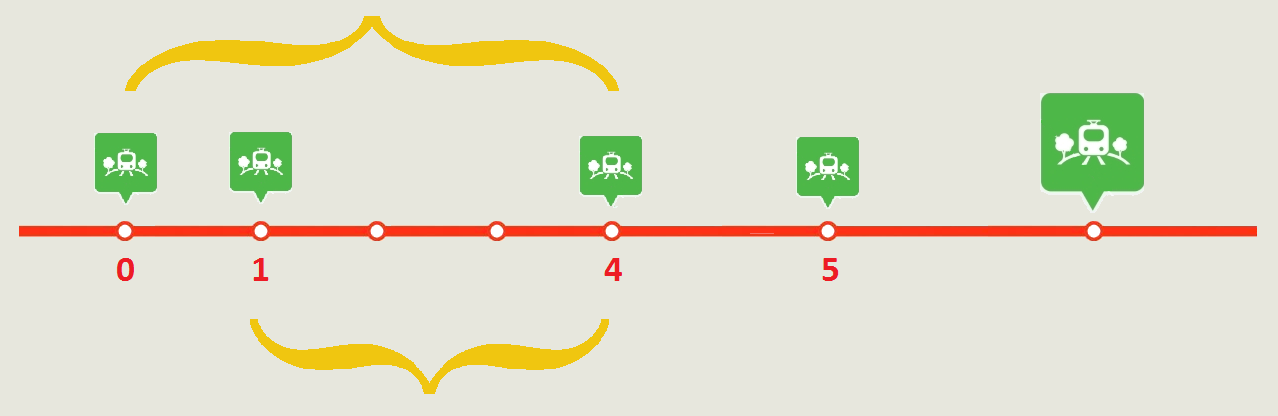
\includegraphics[scale=0.5]{imagenes/ej1/estaciones.png}
	\label{estaciones}
   \end{center}
 \end{figure}

Un algoritmo planteado a partir de esta idea, partiría de la estación Nro. 0 para concluir que se pueden conectar todas desde aquella hasta la Nro 4, para luego continuar revisando una a una las estaciones que pueden unirse partiendo de la Nro 1, cuando resulta evidente que si la distancia entre las estaciones  0 y 4 es menor o igual a la longitud del cable entonces necesariamente la distancia entre la estación siguiente (la Nro. 1) y la Nro. 4 también será menor a la longitud del cable. De no considerar esta premisa se desprende la redundancia en los cálculos que impactan en la complejidad de algoritmo. \\
 
Dicho esto, la propuesta de resolución escogida versa sobre la idea de utilizar información relevada en estaciones anteriores para aminorar la cantidad de cómputos, como se esboza en el siguiente pseudocódigo:


\begin{algorithmic} 
	
\IF{Existe alguna estación en el ramal y la longitud del cable es positiva}
	\WHILE{La estación a partir de la cuál estoy midiendo no es la última y tapoco lo es la más lejana alcanzada por dicha estación}
		\STATE Calcular la cantidad de ciudades para las cuales se sabe que alcanza el cable
		\WHILE{Alcanza el cable para unir otra estación}
			\STATE Incrementar la cantidad de estaciones que pudieron unirse
			\STATE Guardar cuál fue la estación más lejana alcanzada hasta el momento a partir de la que se mide
		\ENDWHILE
		\STATE Avanzar ciudad a partir de la cuál se mide
		\STATE Actualizar la máxima cantidad de ciudades unidas hasta el momento.
	\ENDWHILE
	\IF {Se lograron conectar dos o más ciudades}
		\STATE Devolver la maxima cantidad de estaciones que se consiguió unir.
	\ELSE
		\STATE Devolver 0
	\ENDIF
\ENDIF
\end{algorithmic}

Este procedimiento resuelve adecuadamente el problema propuesto porque calcula para cada ciudad inicial la máxima cantidad de ciudades que pueden ser recorridas y lo realiza con una cota de complejidad de O(n), como se detallará en el próximo apartado.\\
Además, como se afirma que un programa es correcto si resuelve lo pedido en una cantidad finita de pasos y sabiendo que para cualquier entrada de tama\~no N el algoritmo termina a lo sumo en $m*N$ interaciones del loop principal (con m un entero positivo) \footnote{Nótese que el bucle principal llega a su fin cuando se alcanza como ciudad base a la última estación de un ramal de N estaciones que se recorre linealmente}, podemos afirmar que nuestra solución es correcta respecto del problema presentado.\\

\newpage
\subsection{An\'alisis de la complejidad}


Sea N la cantidad total de estaciones \\

Entonces se afirma que en el peor caso cada estación va a ser estación basal en alguna instanciación del ciclo. En otras palabras, el ciclo se repetirá a lo sumo N veces.\\
Dada una instanciación del ciclo en la estación i-ésima ($i != 0$), existen dos posibilidades:
\begin{itemize}
\item	La estación $i-1$ llegó a conectar a la i-ésima y a $k$ estaciones posteriores a ella.
\item	El cable no fue lo suficientemente largo para lograrlo.
\end{itemize}

Si nos encontráramos en el segundo caso, el algoritmo partiría de la ciudad i-ésima recorriendo a lo sumo $N-i-1$ estaciones posteriores para analizar hasta cuál es capaz de unir.\\
Si el caso fuese el primero, entonces la ciudad posterior ($i$) contrastará la longitud del cable y las distancias entre kilometros para - a lo sumo - N-i-1-k estaciones (en lugar de hacerlo para N-i-1, como hubiese debido hacerlo bajo otras circunstancias).\\

Esto implica que para cada estación $i$, podrían llegar a realizarse a lo sumo N-i-1 comparaciones pero todas aquellas que se efectúen serán descontadas de la cantidad de cálculos que potencialmente haría la ciudad siguiente, forzando a que cada estación sea consultada acerca de su proximidad una sola vez y permitiendo de esta manera que la ejecución del algoritmo se complete en tiempo lineal respecto del tamaño del input.\\ 

 \newpage
\subsection{C\'odigo fuente}

A continuación se presenta la parte más relevante del código fuente, seleccionada en función de la relación con la resolución del problema, dejando de lado aspectos necesarios pero secundarios, como ser el manejo de la lectura del input, la escritura del output, 
la medición de los tiempos, etc.

\begin{verbatim}

public class Main 
{
  public static void main(String[] args) throws Exception 
  {
 
	if (longitudCable != 0 && ciudades.size() > 1)
	{
	    Ramal ramal = new Ramal(ciudades);
	    int indiceCiudadMasLejanaAlcanzada    = 0;  
	    int cantMaximaCiudadesUnidas          = 1;   
	    int ciudadesUnidas;

	    while(ramal.HayCiudadesMasLejanas() &&
		 !ramal.EsLaUltimaCiudad(indiceCiudadMasLejanaAlcanzada)) 
	    {
	        if (indiceCiudadMasLejanaAlcanzada > ramal.indiceCiudadActual)
	            ciudadesUnidas =  indiceCiudadMasLejanaAlcanzada -
					 ramal.indiceCiudadActual + 1;
	        else
	            ciudadesUnidas = 1;                 

	        while(ramal.AlcanzaParaUnirUnaCiudadMas(ciudadesUnidas, longitudCable)) 
	        {
	            ciudadesUnidas ++;
	            indiceCiudadMasLejanaAlcanzada ++;
	        }
	                                
	        ramal.AvanzarCiudadBase();
	        
	        if (ciudadesUnidas > cantMaximaCiudadesUnidas)
	            cantMaximaCiudadesUnidas = ciudadesUnidas;
	        
	    }
	      
	    res = cantMaximaCiudadesUnidas == 1? 0: cantMaximaCiudadesUnidas;

	}
	else
	{
	    res = 0;
	}
  } 
}

\end{verbatim}

\newpage
\begin{verbatim}

public class Ramal {
	
    public Ramal(){}

	public ArrayList<Ciudad> ciudades;

	public Ramal (ArrayList<Ciudad> ciudades)
	{
		this.ciudades = ciudades;
		this.indiceCiudadActual = 0;
	}
	
	public int indiceCiudadActual;
	
	public boolean AlcanzaParaUnirUnaCiudadMas(int ciudadesUnidas, int longitudDeCable) 
	{
		return !EsLaUltimaCiudad(indiceCiudadActual) &&
		!EsLaUltimaCiudad(indiceCiudadActual + ciudadesUnidas - 1) &&
		DistanciaEntreCiudades(indiceCiudadActual, indiceCiudadActual + ciudadesUnidas) 
											<= longitudDeCable; 
	}
	
	public void AvanzarCiudadBase()
	{
		if (!EsLaUltimaCiudad(indiceCiudadActual))
			indiceCiudadActual++;
	}
	
	public boolean HayCiudadesMasLejanas()
	{
		return (indiceCiudadActual < ciudades.size() - 1);
	}
	
	public int DistanciaEntreCiudades(int indiceCiudadA, int indiceCiudadB)
	{
		return this.ciudades.get(indiceCiudadB).GetKilometro() -
			 this.ciudades.get(indiceCiudadA).GetKilometro();
	}

	public boolean EsLaUltimaCiudad(int indiceCiudad) 
	{
		return indiceCiudad == this.ciudades.size() - 1;
	}
}

\end{verbatim}
\newpage
\subsection{Experimentaci\'on}

Para contrastar nuestra hipótesis acerca de la complejidad temporal lineal del algoritmo propuesto, diseñamos una clase denominada ClassGenerator1 encargada de generar ramales pseudoaleatorios con una cantidad de estaciones secuencialmente creciente.\\ 
La misma clase ejecuta sobre cada instancia una cantidad paramétrica de veces \footnote{350 veces, en este caso} el algoritmo que resuelve el problema propuesto. Por cada iteración sobre una misma instancia se guardan los tiempos medidos y al finalizar todas las ejecuciones sobre cada una de las instancias, se almacena en un archivo denominado "resultados.out" el procesamiento de los datos relevados, de manera tal que persista para cada caso el promedio de los tiempos calculados sin considerar los outliers.\\
De esta forma procuramos estandarizar en la medida de lo posible los resultados, de manera que no resulten considerablemente afectados por limitaciones del hardware y del software empleado durante el análisis. \\
 \newpage

\subsubsection{Constrastaci\'on Emp\'irica de la complejidad}

  \begin{figure}[h!]
   \begin{center}
 	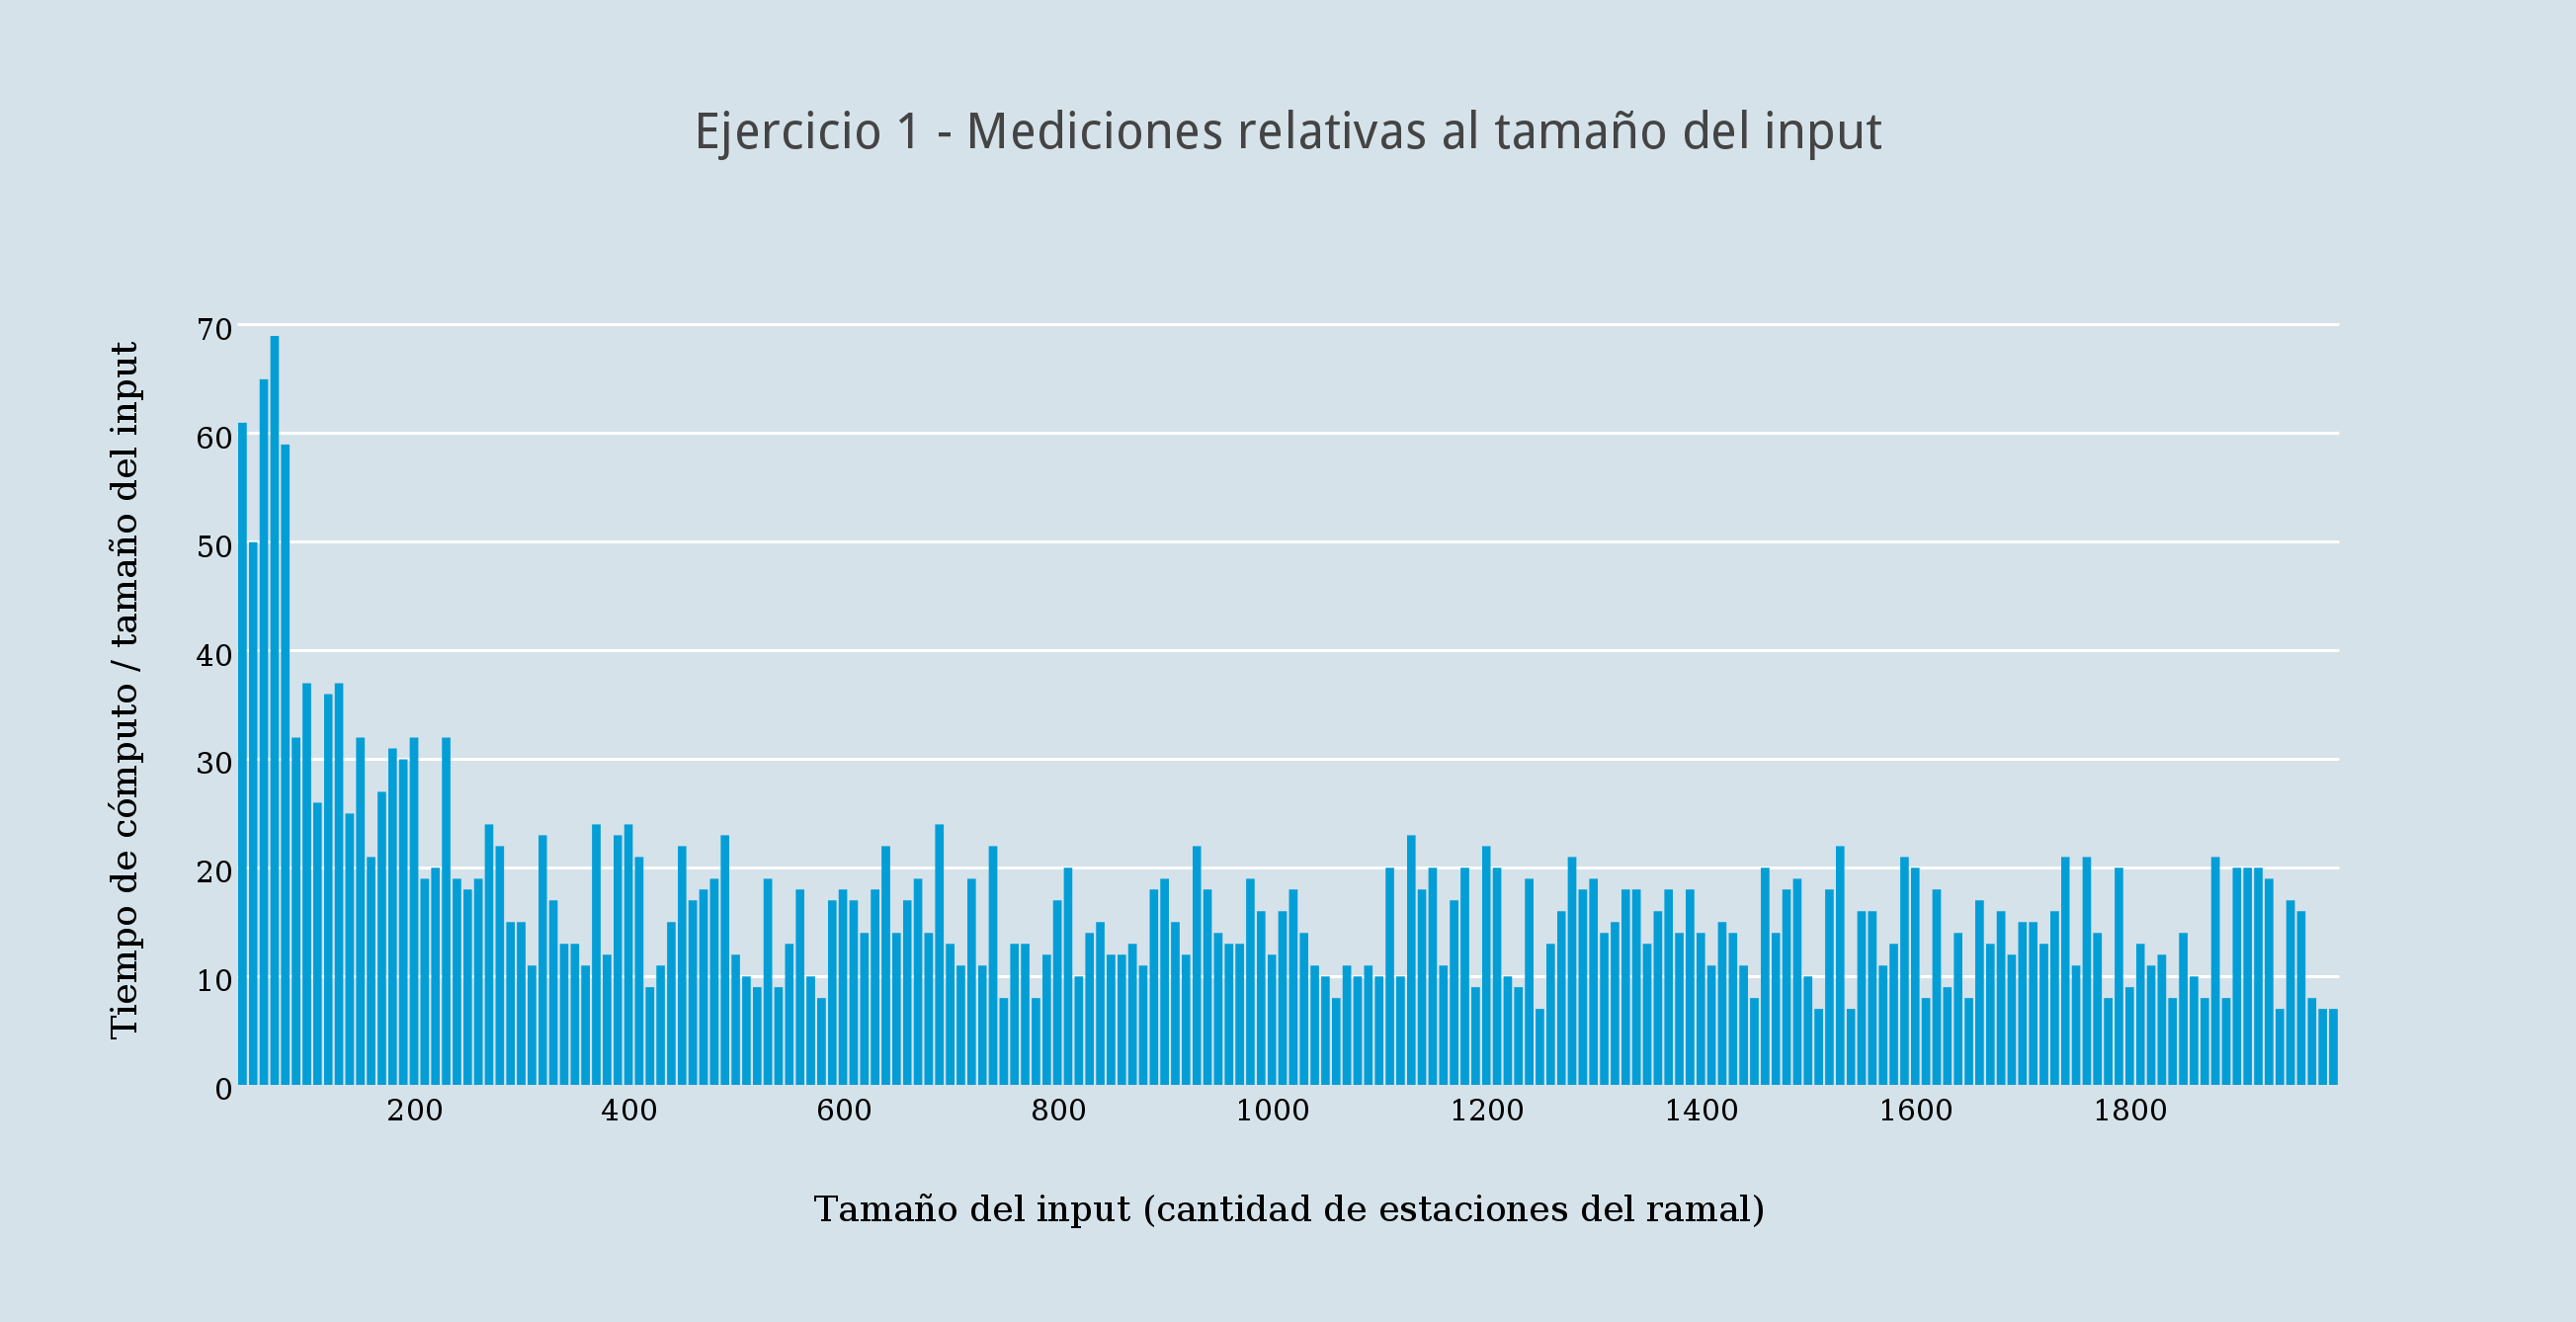
\includegraphics[scale=0.8]{imagenes/ej1/relativas.png}
	\label{estaciones}
   \end{center}
 \end{figure}

  \begin{figure}[h!]
   \begin{center}
 	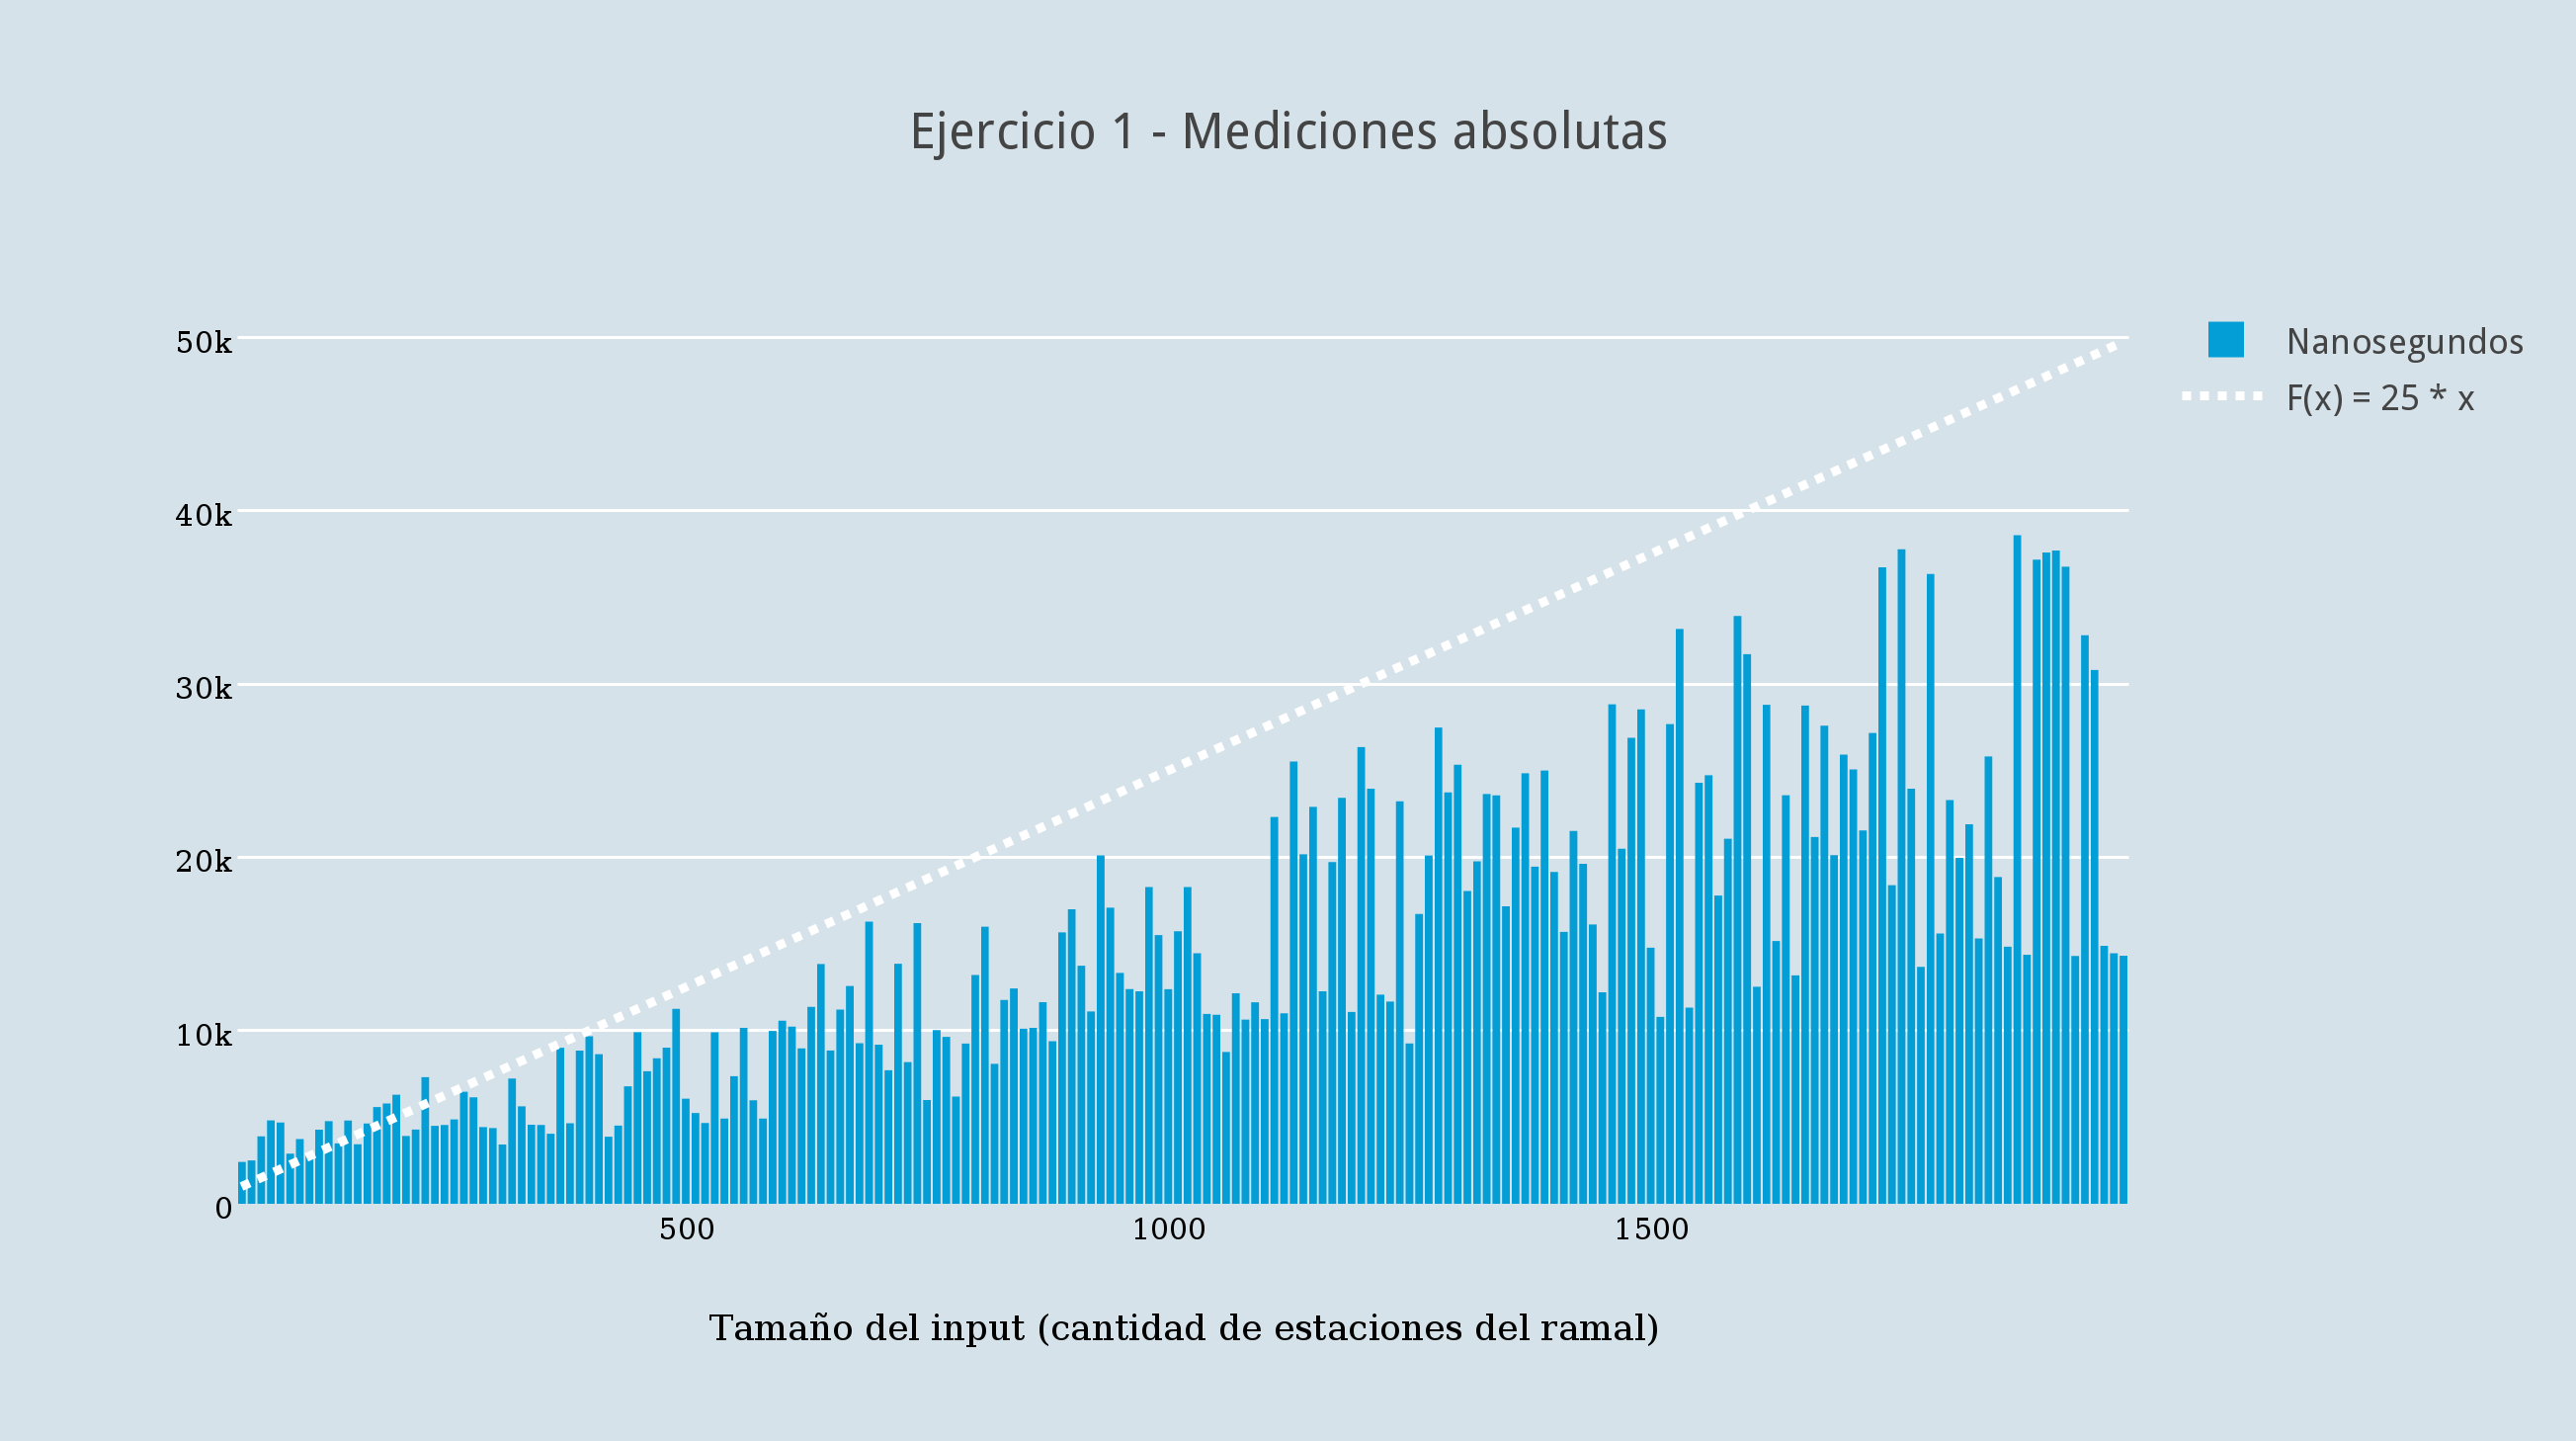
\includegraphics[scale=0.8]{imagenes/ej1/absolutas.png}
	\label{estaciones}
   \end{center}
 \end{figure}


\newpage

{\huge \textcolor{blue}{Fijarse en los casos en que el tiempo es menor al esperado, cuál es el motivo (si es que hay algún caso que se repita). Completar argumentación viendo que el puntero sólo va hacia adelante.}}
